\documentclass[twoside]{book}

% Packages required by doxygen
\usepackage{calc}
\usepackage{doxygen}
\usepackage{graphicx}
\usepackage[utf8]{inputenc}
\usepackage{makeidx}
\usepackage{multicol}
\usepackage{multirow}
\usepackage{textcomp}
\usepackage[table]{xcolor}

% Font selection
\usepackage[T1]{fontenc}
\usepackage{mathptmx}
\usepackage[scaled=.90]{helvet}
\usepackage{courier}
\usepackage{amssymb}
\usepackage{sectsty}
\renewcommand{\familydefault}{\sfdefault}
\allsectionsfont{%
  \fontseries{bc}\selectfont%
  \color{darkgray}%
}
\renewcommand{\DoxyLabelFont}{%
  \fontseries{bc}\selectfont%
  \color{darkgray}%
}

% Page & text layout
\usepackage{geometry}
\geometry{%
  a4paper,%
  top=2.5cm,%
  bottom=2.5cm,%
  left=2.5cm,%
  right=2.5cm%
}
\tolerance=750
\hfuzz=15pt
\hbadness=750
\setlength{\emergencystretch}{15pt}
\setlength{\parindent}{0cm}
\setlength{\parskip}{0.2cm}
\makeatletter
\renewcommand{\paragraph}{%
  \@startsection{paragraph}{4}{0ex}{-1.0ex}{1.0ex}{%
    \normalfont\normalsize\bfseries\SS@parafont%
  }%
}
\renewcommand{\subparagraph}{%
  \@startsection{subparagraph}{5}{0ex}{-1.0ex}{1.0ex}{%
    \normalfont\normalsize\bfseries\SS@subparafont%
  }%
}
\makeatother

% Headers & footers
\usepackage{fancyhdr}
\pagestyle{fancyplain}
\fancyhead[LE]{\fancyplain{}{\bfseries\thepage}}
\fancyhead[CE]{\fancyplain{}{}}
\fancyhead[RE]{\fancyplain{}{\bfseries\leftmark}}
\fancyhead[LO]{\fancyplain{}{\bfseries\rightmark}}
\fancyhead[CO]{\fancyplain{}{}}
\fancyhead[RO]{\fancyplain{}{\bfseries\thepage}}
\fancyfoot[LE]{\fancyplain{}{}}
\fancyfoot[CE]{\fancyplain{}{}}
\fancyfoot[RE]{\fancyplain{}{\bfseries\scriptsize Generated on Tue Oct 24 2017 02\-:54\-:34 for My Project by Doxygen }}
\fancyfoot[LO]{\fancyplain{}{\bfseries\scriptsize Generated on Tue Oct 24 2017 02\-:54\-:34 for My Project by Doxygen }}
\fancyfoot[CO]{\fancyplain{}{}}
\fancyfoot[RO]{\fancyplain{}{}}
\renewcommand{\footrulewidth}{0.4pt}
\renewcommand{\chaptermark}[1]{%
  \markboth{#1}{}%
}
\renewcommand{\sectionmark}[1]{%
  \markright{\thesection\ #1}%
}

% Indices & bibliography
\usepackage{natbib}
\usepackage[titles]{tocloft}
\setcounter{tocdepth}{3}
\setcounter{secnumdepth}{5}
\makeindex

% Hyperlinks (required, but should be loaded last)
\usepackage{ifpdf}
\ifpdf
  \usepackage[pdftex,pagebackref=true]{hyperref}
\else
  \usepackage[ps2pdf,pagebackref=true]{hyperref}
\fi
\hypersetup{%
  colorlinks=true,%
  linkcolor=blue,%
  citecolor=blue,%
  unicode%
}

% Custom commands
\newcommand{\clearemptydoublepage}{%
  \newpage{\pagestyle{empty}\cleardoublepage}%
}


%===== C O N T E N T S =====

\begin{document}

% Titlepage & ToC
\hypersetup{pageanchor=false}
\pagenumbering{roman}
\begin{titlepage}
\vspace*{7cm}
\begin{center}%
{\Large My Project }\\
\vspace*{1cm}
{\large Generated by Doxygen 1.8.6}\\
\vspace*{0.5cm}
{\small Tue Oct 24 2017 02:54:34}\\
\end{center}
\end{titlepage}
\clearemptydoublepage
\tableofcontents
\clearemptydoublepage
\pagenumbering{arabic}
\hypersetup{pageanchor=true}

%--- Begin generated contents ---
\chapter{Class Index}
\section{Class List}
Here are the classes, structs, unions and interfaces with brief descriptions\-:\begin{DoxyCompactList}
\item\contentsline{section}{\hyperlink{classcmd__vel__joystick}{cmd\-\_\-vel\-\_\-joystick} }{\pageref{classcmd__vel__joystick}}{}
\item\contentsline{section}{\hyperlink{classControl}{Control} }{\pageref{classControl}}{}
\item\contentsline{section}{\hyperlink{structControl_1_1Pose}{Control\-::\-Pose} \\*The \hyperlink{structControl_1_1Pose}{Pose} include the 2 d x and x position and the heading th }{\pageref{structControl_1_1Pose}}{}
\end{DoxyCompactList}

\chapter{File Index}
\section{File List}
Here is a list of all files with brief descriptions\-:\begin{DoxyCompactList}
\item\contentsline{section}{include/\hyperlink{Control_8h}{Control.\-h} }{\pageref{Control_8h}}{}
\item\contentsline{section}{src/\hyperlink{cmd__joy_8cpp}{cmd\-\_\-joy.\-cpp} }{\pageref{cmd__joy_8cpp}}{}
\item\contentsline{section}{src/\hyperlink{Control_8cpp}{Control.\-cpp} }{\pageref{Control_8cpp}}{}
\end{DoxyCompactList}

\chapter{Class Documentation}
\hypertarget{classcmd__vel__joystick}{\section{cmd\-\_\-vel\-\_\-joystick Class Reference}
\label{classcmd__vel__joystick}\index{cmd\-\_\-vel\-\_\-joystick@{cmd\-\_\-vel\-\_\-joystick}}
}
\subsection*{Public Member Functions}
\begin{DoxyCompactItemize}
\item 
\hyperlink{classcmd__vel__joystick_af0e18e4b1bb5fcac03585e8ffde8e38d}{cmd\-\_\-vel\-\_\-joystick} ()
\end{DoxyCompactItemize}
\subsection*{Private Member Functions}
\begin{DoxyCompactItemize}
\item 
void \hyperlink{classcmd__vel__joystick_a22571f85861dfa5631f68b8e8e6d0497}{joy\-Callback} (const sensor\-\_\-msgs\-::\-Joy\-::\-Const\-Ptr \&joy)
\end{DoxyCompactItemize}
\subsection*{Private Attributes}
\begin{DoxyCompactItemize}
\item 
ros\-::\-Node\-Handle \hyperlink{classcmd__vel__joystick_ae50ce40991b7bfff45a21adbfc028465}{node\-Handle}
\item 
ros\-::\-Publisher \hyperlink{classcmd__vel__joystick_a8c089e3c358de60bd10ab17a2553dc44}{cmd\-\_\-vel\-\_\-pub}
\item 
ros\-::\-Subscriber \hyperlink{classcmd__vel__joystick_a2947a21136647b829b50058c0ced8b01}{joy\-\_\-sub}
\item 
geometry\-\_\-msgs\-::\-Twist \hyperlink{classcmd__vel__joystick_a8f909c2268739f4aad576786c8876576}{cmd\-\_\-vel}
\item 
int \hyperlink{classcmd__vel__joystick_a24f26021bde377287c5790dc5f734cc5}{robot\-\_\-drive\-\_\-dir}
\end{DoxyCompactItemize}


\subsection{Detailed Description}


Definition at line 11 of file cmd\-\_\-joy.\-cpp.



\subsection{Constructor \& Destructor Documentation}
\hypertarget{classcmd__vel__joystick_af0e18e4b1bb5fcac03585e8ffde8e38d}{\index{cmd\-\_\-vel\-\_\-joystick@{cmd\-\_\-vel\-\_\-joystick}!cmd\-\_\-vel\-\_\-joystick@{cmd\-\_\-vel\-\_\-joystick}}
\index{cmd\-\_\-vel\-\_\-joystick@{cmd\-\_\-vel\-\_\-joystick}!cmd_vel_joystick@{cmd\-\_\-vel\-\_\-joystick}}
\subsubsection[{cmd\-\_\-vel\-\_\-joystick}]{\setlength{\rightskip}{0pt plus 5cm}cmd\-\_\-vel\-\_\-joystick\-::cmd\-\_\-vel\-\_\-joystick (
\begin{DoxyParamCaption}
{}
\end{DoxyParamCaption}
)}}\label{classcmd__vel__joystick_af0e18e4b1bb5fcac03585e8ffde8e38d}


Definition at line 26 of file cmd\-\_\-joy.\-cpp.



\subsection{Member Function Documentation}
\hypertarget{classcmd__vel__joystick_a22571f85861dfa5631f68b8e8e6d0497}{\index{cmd\-\_\-vel\-\_\-joystick@{cmd\-\_\-vel\-\_\-joystick}!joy\-Callback@{joy\-Callback}}
\index{joy\-Callback@{joy\-Callback}!cmd_vel_joystick@{cmd\-\_\-vel\-\_\-joystick}}
\subsubsection[{joy\-Callback}]{\setlength{\rightskip}{0pt plus 5cm}void cmd\-\_\-vel\-\_\-joystick\-::joy\-Callback (
\begin{DoxyParamCaption}
\item[{const sensor\-\_\-msgs\-::\-Joy\-::\-Const\-Ptr \&}]{joy}
\end{DoxyParamCaption}
)\hspace{0.3cm}{\ttfamily [private]}}}\label{classcmd__vel__joystick_a22571f85861dfa5631f68b8e8e6d0497}


Definition at line 43 of file cmd\-\_\-joy.\-cpp.



\subsection{Member Data Documentation}
\hypertarget{classcmd__vel__joystick_a8f909c2268739f4aad576786c8876576}{\index{cmd\-\_\-vel\-\_\-joystick@{cmd\-\_\-vel\-\_\-joystick}!cmd\-\_\-vel@{cmd\-\_\-vel}}
\index{cmd\-\_\-vel@{cmd\-\_\-vel}!cmd_vel_joystick@{cmd\-\_\-vel\-\_\-joystick}}
\subsubsection[{cmd\-\_\-vel}]{\setlength{\rightskip}{0pt plus 5cm}geometry\-\_\-msgs\-::\-Twist cmd\-\_\-vel\-\_\-joystick\-::cmd\-\_\-vel\hspace{0.3cm}{\ttfamily [private]}}}\label{classcmd__vel__joystick_a8f909c2268739f4aad576786c8876576}


Definition at line 21 of file cmd\-\_\-joy.\-cpp.

\hypertarget{classcmd__vel__joystick_a8c089e3c358de60bd10ab17a2553dc44}{\index{cmd\-\_\-vel\-\_\-joystick@{cmd\-\_\-vel\-\_\-joystick}!cmd\-\_\-vel\-\_\-pub@{cmd\-\_\-vel\-\_\-pub}}
\index{cmd\-\_\-vel\-\_\-pub@{cmd\-\_\-vel\-\_\-pub}!cmd_vel_joystick@{cmd\-\_\-vel\-\_\-joystick}}
\subsubsection[{cmd\-\_\-vel\-\_\-pub}]{\setlength{\rightskip}{0pt plus 5cm}ros\-::\-Publisher cmd\-\_\-vel\-\_\-joystick\-::cmd\-\_\-vel\-\_\-pub\hspace{0.3cm}{\ttfamily [private]}}}\label{classcmd__vel__joystick_a8c089e3c358de60bd10ab17a2553dc44}


Definition at line 18 of file cmd\-\_\-joy.\-cpp.

\hypertarget{classcmd__vel__joystick_a2947a21136647b829b50058c0ced8b01}{\index{cmd\-\_\-vel\-\_\-joystick@{cmd\-\_\-vel\-\_\-joystick}!joy\-\_\-sub@{joy\-\_\-sub}}
\index{joy\-\_\-sub@{joy\-\_\-sub}!cmd_vel_joystick@{cmd\-\_\-vel\-\_\-joystick}}
\subsubsection[{joy\-\_\-sub}]{\setlength{\rightskip}{0pt plus 5cm}ros\-::\-Subscriber cmd\-\_\-vel\-\_\-joystick\-::joy\-\_\-sub\hspace{0.3cm}{\ttfamily [private]}}}\label{classcmd__vel__joystick_a2947a21136647b829b50058c0ced8b01}


Definition at line 19 of file cmd\-\_\-joy.\-cpp.

\hypertarget{classcmd__vel__joystick_ae50ce40991b7bfff45a21adbfc028465}{\index{cmd\-\_\-vel\-\_\-joystick@{cmd\-\_\-vel\-\_\-joystick}!node\-Handle@{node\-Handle}}
\index{node\-Handle@{node\-Handle}!cmd_vel_joystick@{cmd\-\_\-vel\-\_\-joystick}}
\subsubsection[{node\-Handle}]{\setlength{\rightskip}{0pt plus 5cm}ros\-::\-Node\-Handle cmd\-\_\-vel\-\_\-joystick\-::node\-Handle\hspace{0.3cm}{\ttfamily [private]}}}\label{classcmd__vel__joystick_ae50ce40991b7bfff45a21adbfc028465}


Definition at line 17 of file cmd\-\_\-joy.\-cpp.

\hypertarget{classcmd__vel__joystick_a24f26021bde377287c5790dc5f734cc5}{\index{cmd\-\_\-vel\-\_\-joystick@{cmd\-\_\-vel\-\_\-joystick}!robot\-\_\-drive\-\_\-dir@{robot\-\_\-drive\-\_\-dir}}
\index{robot\-\_\-drive\-\_\-dir@{robot\-\_\-drive\-\_\-dir}!cmd_vel_joystick@{cmd\-\_\-vel\-\_\-joystick}}
\subsubsection[{robot\-\_\-drive\-\_\-dir}]{\setlength{\rightskip}{0pt plus 5cm}int cmd\-\_\-vel\-\_\-joystick\-::robot\-\_\-drive\-\_\-dir\hspace{0.3cm}{\ttfamily [private]}}}\label{classcmd__vel__joystick_a24f26021bde377287c5790dc5f734cc5}


Definition at line 23 of file cmd\-\_\-joy.\-cpp.



The documentation for this class was generated from the following file\-:\begin{DoxyCompactItemize}
\item 
src/\hyperlink{cmd__joy_8cpp}{cmd\-\_\-joy.\-cpp}\end{DoxyCompactItemize}

\hypertarget{classControl}{\section{Control Class Reference}
\label{classControl}\index{Control@{Control}}
}


{\ttfamily \#include $<$Control.\-h$>$}



Collaboration diagram for Control\-:\nopagebreak
\begin{figure}[H]
\begin{center}
\leavevmode
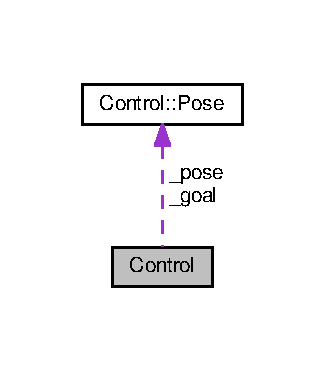
\includegraphics[width=156pt]{classControl__coll__graph}
\end{center}
\end{figure}
\subsection*{Classes}
\begin{DoxyCompactItemize}
\item 
struct \hyperlink{structControl_1_1Pose}{Pose}
\begin{DoxyCompactList}\small\item\em The \hyperlink{structControl_1_1Pose}{Pose} include the 2 d x and x position and the heading th. \end{DoxyCompactList}\end{DoxyCompactItemize}
\subsection*{Public Member Functions}
\begin{DoxyCompactItemize}
\item 
double \hyperlink{classControl_a775cd16905c89b9976935c0fcac16819}{get\-Distance} ()
\item 
\hyperlink{classControl_a497563ec0593b497d2611c1fc49e46db}{Control} (ros\-::\-Node\-Handle n)
\item 
\hyperlink{classControl_aedda1328c4f8b8d49bca8f0812d3bfd1}{$\sim$\-Control} ()
\item 
void \hyperlink{classControl_a26712b5c951b7867390ddcc6b0dd8dce}{get\-Command} (const geometry\-\_\-msgs\-::\-Twist \&msg)
\item 
void \hyperlink{classControl_a533326e0d21ff3d104495d6bd34a6300}{get\-Sensor\-Data} (const nxt\-\_\-control\-::\-Sensor\-Data \&msg)
\item 
geometry\-\_\-msgs\-::\-Pose\-With\-Covariance\-Stamped \hyperlink{classControl_a76545b2751f147c71760c98620e96cdc}{publish\-Odometry} ()
\item 
void \hyperlink{classControl_a2e30ee0e4acae0c6f9266bd94fea679e}{set\-Initial\-Pose} (const geometry\-\_\-msgs\-::\-Pose\-With\-Covariance \&msg)
\end{DoxyCompactItemize}
\subsection*{Private Member Functions}
\begin{DoxyCompactItemize}
\item 
nxt\-\_\-control\-::\-Motor\-Command \hyperlink{classControl_a5b7c8066cc7de499d5a5f6727f975b63}{publish\-Effort} (const geometry\-\_\-msgs\-::\-Twist \&msg, double th\-\_\-speed)
\item 
void \hyperlink{classControl_ae4d44c4c8a9a322c8d7cb0e84e408c74}{update\-Position} (const nxt\-\_\-control\-::\-Sensor\-Data \&msg)
\item 
geometry\-\_\-msgs\-::\-Pose\-With\-Covariance\-Stamped \hyperlink{classControl_a30aa3c2a10b629e35f8e0b86c8e9cb8c}{publish\-Odom} ()
\item 
void \hyperlink{classControl_a8ee4dbe468dc391360c69b45d5af1fb1}{norm\-Speed\-To} (double \&speed1, double \&speed2, double maxspeed)
\item 
nxt\-\_\-control\-::\-Motor\-Command \hyperlink{classControl_aa031d7a2017458e7181a38cd6f403de0}{pub\-Stop} ()
\item 
bool \hyperlink{classControl_a228637543b285e4fd0caf2ec0ceacd7a}{goal\-\_\-reached} (double x, double y, double th)
\item 
sensor\-\_\-msgs\-::\-Range \hyperlink{classControl_a8f688474b0a6e43ba50e5e22eea6d336}{publish\-Ultrasonic\-Range} (const nxt\-\_\-control\-::\-Sensor\-Data \&msg)
\end{DoxyCompactItemize}
\subsection*{Private Attributes}
\begin{DoxyCompactItemize}
\item 
\hyperlink{structControl_1_1Pose}{Pose} \hyperlink{classControl_a55028ed5b7ee32c69282a3e51a7d63f1}{\-\_\-goal}
\begin{DoxyCompactList}\small\item\em Goal pose is calculated from actual pose + velocity command. \end{DoxyCompactList}\item 
\hyperlink{structControl_1_1Pose}{Pose} \hyperlink{classControl_a5aaf886a6c03a01a66b1d692ee0194ae}{\-\_\-pose}
\begin{DoxyCompactList}\small\item\em Actual pose of the robot. \end{DoxyCompactList}\item 
ros\-::\-Node\-Handle \hyperlink{classControl_a535634dd1aa6331c1da87a3da4800fac}{\-\_\-n}
\begin{DoxyCompactList}\small\item\em Ros node handle. \end{DoxyCompactList}\item 
ros\-::\-Publisher \hyperlink{classControl_ae82077fb676becf3f23fd0d87b5b818c}{pub\-Odom}
\begin{DoxyCompactList}\small\item\em publish the position default tiopic\-:odom. \end{DoxyCompactList}\item 
ros\-::\-Publisher \hyperlink{classControl_a9e46e0589c03e37f3ade64d617e2d89c}{pub\-Ultrasonic}
\begin{DoxyCompactList}\small\item\em publish the ultrasonic range measurement in the \char`\"{}ultrasonic\char`\"{} frame default topic\-:ultrasonic \end{DoxyCompactList}\item 
ros\-::\-Publisher \hyperlink{classControl_a3aaa95c82a13bc4d25aa983ec875f31f}{pub\-Effort}
\item 
ros\-::\-Subscriber \hyperlink{classControl_a497d6d472f41ae3e087e8d7ea4c79e7c}{sub\-Command}
\item 
ros\-::\-Subscriber \hyperlink{classControl_af489d55663df41604322747fe6209c17}{sub\-Sensors}
\item 
ros\-::\-Publisher \hyperlink{classControl_a709f0421b317029ef691d15d18974179}{pub\-Nextcmd}
\item 
double \hyperlink{classControl_a52c40a20af6d88b0ba97b0abf006616b}{\-\_\-axis\-\_\-length}
\item 
double \hyperlink{classControl_a502e3555475215826fc7f9b64ec8e0b2}{\-\_\-wheel\-\_\-radius\-\_\-r}
\item 
double \hyperlink{classControl_a78d7fb070693640585e703bb6f626cd1}{\-\_\-gear\-\_\-ratio\-\_\-right}
\begin{DoxyCompactList}\small\item\em Ration between command and right motor effort. \end{DoxyCompactList}\item 
double \hyperlink{classControl_a754081ecec9e1e75fc6df94c22d9df3e}{\-\_\-wheel\-\_\-radius\-\_\-l}
\item 
double \hyperlink{classControl_ad8c978657de600386fc66f935859e095}{\-\_\-gear\-\_\-ratio\-\_\-left}
\begin{DoxyCompactList}\small\item\em Ration between command and right motor effort. \end{DoxyCompactList}\item 
double \hyperlink{classControl_acc9c73871491bc8ac005980ae81d9410}{\-\_\-enc\-\_\-per\-\_\-turn\-\_\-left}
\begin{DoxyCompactList}\small\item\em encounter per turn left wheel \end{DoxyCompactList}\item 
double \hyperlink{classControl_a9f09be60ba816c6c3fb91c47129d2cd1}{\-\_\-enc\-\_\-per\-\_\-turn\-\_\-right}
\begin{DoxyCompactList}\small\item\em encounter per turn right wheel \end{DoxyCompactList}\item 
double \hyperlink{classControl_abcfbef74fbe58b4c24efd11e1c7364f5}{\-\_\-turning\-\_\-adaptation}
\begin{DoxyCompactList}\small\item\em Adjustment for difference between left and right turning. \end{DoxyCompactList}\item 
double \hyperlink{classControl_a1807356ca5230aca9ccb77bf869f007a}{\-\_\-tol\-Trans}
\begin{DoxyCompactList}\small\item\em Tolerance for the position. \end{DoxyCompactList}\item 
double \hyperlink{classControl_ae76716c78a0337c965ff496f9e0ae1fd}{\-\_\-tol\-Rot}
\begin{DoxyCompactList}\small\item\em Tolerance for the heading. \end{DoxyCompactList}\item 
bool \hyperlink{classControl_a3453d34c9b9f47445c0eabc0f774093c}{\-\_\-goal\-\_\-reached}
\item 
double \hyperlink{classControl_ab80522a9174a2af4a37fe8a4ba6ca6d0}{\-\_\-max\-\_\-speed}
\item 
double \hyperlink{classControl_adc6737dda1cb8b841b486e77d5b3b93c}{\-\_\-min\-\_\-speed}
\item 
double \hyperlink{classControl_a2864230e3525ef542b9f3c2c3e91f9aa}{\-\_\-max\-\_\-turn\-\_\-speed}
\item 
double \hyperlink{classControl_a1c3805dd46c4de62a6209bf5ed6b3b93}{\-\_\-distance}
\end{DoxyCompactItemize}


\subsection{Detailed Description}
The \hyperlink{classControl}{Control} class takes care about the communication with a Nxt-\/\-Brick (two motors A\&B and one ultrasonic port 4) The Controler concept is the translation from ros commmon commands to nxt-\/commands. The Controler calculates the Motor\-Commands messages corresponding to a geometry\-\_\-msgs/\-Twist message. The Controler calculates the pose from the ticks of the two Motors and publish a geometry\-\_\-msgs/\-Pose\-With\-Covariance\-Stamped at /odom topic. The Controller publish the ultrasonic measurement as range message in the frame \char`\"{}ultrasonic\char`\"{} 

Definition at line 24 of file Control.\-h.



\subsection{Constructor \& Destructor Documentation}
\hypertarget{classControl_a497563ec0593b497d2611c1fc49e46db}{\index{Control@{Control}!Control@{Control}}
\index{Control@{Control}!Control@{Control}}
\subsubsection[{Control}]{\setlength{\rightskip}{0pt plus 5cm}Control\-::\-Control (
\begin{DoxyParamCaption}
\item[{ros\-::\-Node\-Handle}]{n}
\end{DoxyParamCaption}
)}}\label{classControl_a497563ec0593b497d2611c1fc49e46db}
The constructor registers all subscriber and publisher at a ros node handle The parameter axis\-Length, wheel radius, min/max speed, goal tolerancen gear ration, encounter per tick and a turning adaption are requested from the ros param server or set if they don't exist. 

Definition at line 20 of file Control.\-cpp.

\hypertarget{classControl_aedda1328c4f8b8d49bca8f0812d3bfd1}{\index{Control@{Control}!$\sim$\-Control@{$\sim$\-Control}}
\index{$\sim$\-Control@{$\sim$\-Control}!Control@{Control}}
\subsubsection[{$\sim$\-Control}]{\setlength{\rightskip}{0pt plus 5cm}Control\-::$\sim$\-Control (
\begin{DoxyParamCaption}
{}
\end{DoxyParamCaption}
)}}\label{classControl_aedda1328c4f8b8d49bca8f0812d3bfd1}


Definition at line 261 of file Control.\-cpp.



\subsection{Member Function Documentation}
\hypertarget{classControl_a26712b5c951b7867390ddcc6b0dd8dce}{\index{Control@{Control}!get\-Command@{get\-Command}}
\index{get\-Command@{get\-Command}!Control@{Control}}
\subsubsection[{get\-Command}]{\setlength{\rightskip}{0pt plus 5cm}void Control\-::get\-Command (
\begin{DoxyParamCaption}
\item[{const geometry\-\_\-msgs\-::\-Twist \&}]{msg}
\end{DoxyParamCaption}
)}}\label{classControl_a26712b5c951b7867390ddcc6b0dd8dce}
get\-Command subscribs a geometry\-\_\-msgs/\-Twist to publish the Motor\-Commands. The x translation and the z angular ot the twist messageare interpreted as a radian measure and are convert in motor efforts. This efforts are normalized to an mximum speed, for turn only the speed is adapted. 

Definition at line 98 of file Control.\-cpp.

\hypertarget{classControl_a775cd16905c89b9976935c0fcac16819}{\index{Control@{Control}!get\-Distance@{get\-Distance}}
\index{get\-Distance@{get\-Distance}!Control@{Control}}
\subsubsection[{get\-Distance}]{\setlength{\rightskip}{0pt plus 5cm}double Control\-::get\-Distance (
\begin{DoxyParamCaption}
{}
\end{DoxyParamCaption}
)}}\label{classControl_a775cd16905c89b9976935c0fcac16819}
Subscribe to the Sensor\-Data of the nxt-\/\-Brick, Updates the distance and position of the robot. Send a stop command to the robot if the goal position is reached. 
\begin{DoxyParams}{Parameters}
{\em msg} & nxt\-\_\-control/\-Sensor\-Data Tickcount\-A, Tick\-Count\-B and distance (Port4) \\
\hline
\end{DoxyParams}


Definition at line 240 of file Control.\-cpp.

\hypertarget{classControl_a533326e0d21ff3d104495d6bd34a6300}{\index{Control@{Control}!get\-Sensor\-Data@{get\-Sensor\-Data}}
\index{get\-Sensor\-Data@{get\-Sensor\-Data}!Control@{Control}}
\subsubsection[{get\-Sensor\-Data}]{\setlength{\rightskip}{0pt plus 5cm}void Control\-::get\-Sensor\-Data (
\begin{DoxyParamCaption}
\item[{const nxt\-\_\-control\-::\-Sensor\-Data \&}]{msg}
\end{DoxyParamCaption}
)}}\label{classControl_a533326e0d21ff3d104495d6bd34a6300}
get\-Sensor\-Data subscribs a nxt\-\_\-control/\-Sensordata message to publish position and range message 

Definition at line 175 of file Control.\-cpp.

\hypertarget{classControl_a228637543b285e4fd0caf2ec0ceacd7a}{\index{Control@{Control}!goal\-\_\-reached@{goal\-\_\-reached}}
\index{goal\-\_\-reached@{goal\-\_\-reached}!Control@{Control}}
\subsubsection[{goal\-\_\-reached}]{\setlength{\rightskip}{0pt plus 5cm}bool Control\-::goal\-\_\-reached (
\begin{DoxyParamCaption}
\item[{double}]{x, }
\item[{double}]{y, }
\item[{double}]{th}
\end{DoxyParamCaption}
)\hspace{0.3cm}{\ttfamily [private]}}}\label{classControl_a228637543b285e4fd0caf2ec0ceacd7a}
goal\-\_\-reached checks if a position is near enough to the goal position 
\begin{DoxyParams}[1]{Parameters}
\mbox{\tt in}  & {\em x} & double, x coordinate of the robot \\
\hline
\mbox{\tt in}  & {\em y} & double, y coordinate of the robot \\
\hline
\mbox{\tt in}  & {\em th} & double, theta the heading of the robot \\
\hline
\end{DoxyParams}
\begin{DoxyReturn}{Returns}
returns true is a position is reached else false 
\end{DoxyReturn}


Definition at line 220 of file Control.\-cpp.

\hypertarget{classControl_a8ee4dbe468dc391360c69b45d5af1fb1}{\index{Control@{Control}!norm\-Speed\-To@{norm\-Speed\-To}}
\index{norm\-Speed\-To@{norm\-Speed\-To}!Control@{Control}}
\subsubsection[{norm\-Speed\-To}]{\setlength{\rightskip}{0pt plus 5cm}void Control\-::norm\-Speed\-To (
\begin{DoxyParamCaption}
\item[{double \&}]{speed1, }
\item[{double \&}]{speed2, }
\item[{double}]{maxspeed}
\end{DoxyParamCaption}
)\hspace{0.3cm}{\ttfamily [private]}}}\label{classControl_a8ee4dbe468dc391360c69b45d5af1fb1}


Definition at line 244 of file Control.\-cpp.

\hypertarget{classControl_a5b7c8066cc7de499d5a5f6727f975b63}{\index{Control@{Control}!publish\-Effort@{publish\-Effort}}
\index{publish\-Effort@{publish\-Effort}!Control@{Control}}
\subsubsection[{publish\-Effort}]{\setlength{\rightskip}{0pt plus 5cm}nxt\-\_\-control\-::\-Motor\-Command Control\-::publish\-Effort (
\begin{DoxyParamCaption}
\item[{const geometry\-\_\-msgs\-::\-Twist \&}]{msg, }
\item[{double}]{th\-\_\-speed}
\end{DoxyParamCaption}
)\hspace{0.3cm}{\ttfamily [private]}}}\label{classControl_a5b7c8066cc7de499d5a5f6727f975b63}


Definition at line 137 of file Control.\-cpp.

\hypertarget{classControl_a30aa3c2a10b629e35f8e0b86c8e9cb8c}{\index{Control@{Control}!publish\-Odom@{publish\-Odom}}
\index{publish\-Odom@{publish\-Odom}!Control@{Control}}
\subsubsection[{publish\-Odom}]{\setlength{\rightskip}{0pt plus 5cm}geometry\-\_\-msgs\-::\-Pose\-With\-Covariance\-Stamped Control\-::publish\-Odom (
\begin{DoxyParamCaption}
{}
\end{DoxyParamCaption}
)\hspace{0.3cm}{\ttfamily [private]}}}\label{classControl_a30aa3c2a10b629e35f8e0b86c8e9cb8c}


Definition at line 210 of file Control.\-cpp.

\hypertarget{classControl_a76545b2751f147c71760c98620e96cdc}{\index{Control@{Control}!publish\-Odometry@{publish\-Odometry}}
\index{publish\-Odometry@{publish\-Odometry}!Control@{Control}}
\subsubsection[{publish\-Odometry}]{\setlength{\rightskip}{0pt plus 5cm}geometry\-\_\-msgs\-::\-Pose\-With\-Covariance\-Stamped Control\-::publish\-Odometry (
\begin{DoxyParamCaption}
{}
\end{DoxyParamCaption}
)}}\label{classControl_a76545b2751f147c71760c98620e96cdc}
publish\-Odometry create a odometry message from the pose variable \begin{DoxyReturn}{Returns}
geometry\-\_\-msgs\-::\-Pose\-With\-Covariance\-Stamped at map frame 
\end{DoxyReturn}
\hypertarget{classControl_a8f688474b0a6e43ba50e5e22eea6d336}{\index{Control@{Control}!publish\-Ultrasonic\-Range@{publish\-Ultrasonic\-Range}}
\index{publish\-Ultrasonic\-Range@{publish\-Ultrasonic\-Range}!Control@{Control}}
\subsubsection[{publish\-Ultrasonic\-Range}]{\setlength{\rightskip}{0pt plus 5cm}sensor\-\_\-msgs\-::\-Range Control\-::publish\-Ultrasonic\-Range (
\begin{DoxyParamCaption}
\item[{const nxt\-\_\-control\-::\-Sensor\-Data \&}]{msg}
\end{DoxyParamCaption}
)\hspace{0.3cm}{\ttfamily [private]}}}\label{classControl_a8f688474b0a6e43ba50e5e22eea6d336}
Set the meta information to a ultrasonic scan\-: frame id and time stamp 

Definition at line 162 of file Control.\-cpp.

\hypertarget{classControl_aa031d7a2017458e7181a38cd6f403de0}{\index{Control@{Control}!pub\-Stop@{pub\-Stop}}
\index{pub\-Stop@{pub\-Stop}!Control@{Control}}
\subsubsection[{pub\-Stop}]{\setlength{\rightskip}{0pt plus 5cm}nxt\-\_\-control\-::\-Motor\-Command Control\-::pub\-Stop (
\begin{DoxyParamCaption}
{}
\end{DoxyParamCaption}
)\hspace{0.3cm}{\ttfamily [private]}}}\label{classControl_aa031d7a2017458e7181a38cd6f403de0}


Definition at line 227 of file Control.\-cpp.

\hypertarget{classControl_a2e30ee0e4acae0c6f9266bd94fea679e}{\index{Control@{Control}!set\-Initial\-Pose@{set\-Initial\-Pose}}
\index{set\-Initial\-Pose@{set\-Initial\-Pose}!Control@{Control}}
\subsubsection[{set\-Initial\-Pose}]{\setlength{\rightskip}{0pt plus 5cm}void Control\-::set\-Initial\-Pose (
\begin{DoxyParamCaption}
\item[{const geometry\-\_\-msgs\-::\-Pose\-With\-Covariance \&}]{msg}
\end{DoxyParamCaption}
)}}\label{classControl_a2e30ee0e4acae0c6f9266bd94fea679e}
set\-Initial\-Pose sets the pose of the robot 
\begin{DoxyParams}[1]{Parameters}
\mbox{\tt in}  & {\em const} & geometry\-\_\-msgs\-::\-Pose\-With\-Covariance message enables pose setting via rviz \\
\hline
\end{DoxyParams}
\hypertarget{classControl_ae4d44c4c8a9a322c8d7cb0e84e408c74}{\index{Control@{Control}!update\-Position@{update\-Position}}
\index{update\-Position@{update\-Position}!Control@{Control}}
\subsubsection[{update\-Position}]{\setlength{\rightskip}{0pt plus 5cm}void Control\-::update\-Position (
\begin{DoxyParamCaption}
\item[{const nxt\-\_\-control\-::\-Sensor\-Data \&}]{msg}
\end{DoxyParamCaption}
)\hspace{0.3cm}{\ttfamily [private]}}}\label{classControl_ae4d44c4c8a9a322c8d7cb0e84e408c74}


Definition at line 188 of file Control.\-cpp.



\subsection{Member Data Documentation}
\hypertarget{classControl_a52c40a20af6d88b0ba97b0abf006616b}{\index{Control@{Control}!\-\_\-axis\-\_\-length@{\-\_\-axis\-\_\-length}}
\index{\-\_\-axis\-\_\-length@{\-\_\-axis\-\_\-length}!Control@{Control}}
\subsubsection[{\-\_\-axis\-\_\-length}]{\setlength{\rightskip}{0pt plus 5cm}double Control\-::\-\_\-axis\-\_\-length\hspace{0.3cm}{\ttfamily [private]}}}\label{classControl_a52c40a20af6d88b0ba97b0abf006616b}


Definition at line 51 of file Control.\-h.

\hypertarget{classControl_a1c3805dd46c4de62a6209bf5ed6b3b93}{\index{Control@{Control}!\-\_\-distance@{\-\_\-distance}}
\index{\-\_\-distance@{\-\_\-distance}!Control@{Control}}
\subsubsection[{\-\_\-distance}]{\setlength{\rightskip}{0pt plus 5cm}double Control\-::\-\_\-distance\hspace{0.3cm}{\ttfamily [private]}}}\label{classControl_a1c3805dd46c4de62a6209bf5ed6b3b93}


Definition at line 75 of file Control.\-h.

\hypertarget{classControl_acc9c73871491bc8ac005980ae81d9410}{\index{Control@{Control}!\-\_\-enc\-\_\-per\-\_\-turn\-\_\-left@{\-\_\-enc\-\_\-per\-\_\-turn\-\_\-left}}
\index{\-\_\-enc\-\_\-per\-\_\-turn\-\_\-left@{\-\_\-enc\-\_\-per\-\_\-turn\-\_\-left}!Control@{Control}}
\subsubsection[{\-\_\-enc\-\_\-per\-\_\-turn\-\_\-left}]{\setlength{\rightskip}{0pt plus 5cm}double Control\-::\-\_\-enc\-\_\-per\-\_\-turn\-\_\-left\hspace{0.3cm}{\ttfamily [private]}}}\label{classControl_acc9c73871491bc8ac005980ae81d9410}


encounter per turn left wheel 



Definition at line 59 of file Control.\-h.

\hypertarget{classControl_a9f09be60ba816c6c3fb91c47129d2cd1}{\index{Control@{Control}!\-\_\-enc\-\_\-per\-\_\-turn\-\_\-right@{\-\_\-enc\-\_\-per\-\_\-turn\-\_\-right}}
\index{\-\_\-enc\-\_\-per\-\_\-turn\-\_\-right@{\-\_\-enc\-\_\-per\-\_\-turn\-\_\-right}!Control@{Control}}
\subsubsection[{\-\_\-enc\-\_\-per\-\_\-turn\-\_\-right}]{\setlength{\rightskip}{0pt plus 5cm}double Control\-::\-\_\-enc\-\_\-per\-\_\-turn\-\_\-right\hspace{0.3cm}{\ttfamily [private]}}}\label{classControl_a9f09be60ba816c6c3fb91c47129d2cd1}


encounter per turn right wheel 



Definition at line 62 of file Control.\-h.

\hypertarget{classControl_ad8c978657de600386fc66f935859e095}{\index{Control@{Control}!\-\_\-gear\-\_\-ratio\-\_\-left@{\-\_\-gear\-\_\-ratio\-\_\-left}}
\index{\-\_\-gear\-\_\-ratio\-\_\-left@{\-\_\-gear\-\_\-ratio\-\_\-left}!Control@{Control}}
\subsubsection[{\-\_\-gear\-\_\-ratio\-\_\-left}]{\setlength{\rightskip}{0pt plus 5cm}double Control\-::\-\_\-gear\-\_\-ratio\-\_\-left\hspace{0.3cm}{\ttfamily [private]}}}\label{classControl_ad8c978657de600386fc66f935859e095}


Ration between command and right motor effort. 



Definition at line 57 of file Control.\-h.

\hypertarget{classControl_a78d7fb070693640585e703bb6f626cd1}{\index{Control@{Control}!\-\_\-gear\-\_\-ratio\-\_\-right@{\-\_\-gear\-\_\-ratio\-\_\-right}}
\index{\-\_\-gear\-\_\-ratio\-\_\-right@{\-\_\-gear\-\_\-ratio\-\_\-right}!Control@{Control}}
\subsubsection[{\-\_\-gear\-\_\-ratio\-\_\-right}]{\setlength{\rightskip}{0pt plus 5cm}double Control\-::\-\_\-gear\-\_\-ratio\-\_\-right\hspace{0.3cm}{\ttfamily [private]}}}\label{classControl_a78d7fb070693640585e703bb6f626cd1}


Ration between command and right motor effort. 



Definition at line 54 of file Control.\-h.

\hypertarget{classControl_a55028ed5b7ee32c69282a3e51a7d63f1}{\index{Control@{Control}!\-\_\-goal@{\-\_\-goal}}
\index{\-\_\-goal@{\-\_\-goal}!Control@{Control}}
\subsubsection[{\-\_\-goal}]{\setlength{\rightskip}{0pt plus 5cm}{\bf Pose} Control\-::\-\_\-goal\hspace{0.3cm}{\ttfamily [private]}}}\label{classControl_a55028ed5b7ee32c69282a3e51a7d63f1}


Goal pose is calculated from actual pose + velocity command. 



Definition at line 36 of file Control.\-h.

\hypertarget{classControl_a3453d34c9b9f47445c0eabc0f774093c}{\index{Control@{Control}!\-\_\-goal\-\_\-reached@{\-\_\-goal\-\_\-reached}}
\index{\-\_\-goal\-\_\-reached@{\-\_\-goal\-\_\-reached}!Control@{Control}}
\subsubsection[{\-\_\-goal\-\_\-reached}]{\setlength{\rightskip}{0pt plus 5cm}bool Control\-::\-\_\-goal\-\_\-reached\hspace{0.3cm}{\ttfamily [private]}}}\label{classControl_a3453d34c9b9f47445c0eabc0f774093c}


Definition at line 71 of file Control.\-h.

\hypertarget{classControl_ab80522a9174a2af4a37fe8a4ba6ca6d0}{\index{Control@{Control}!\-\_\-max\-\_\-speed@{\-\_\-max\-\_\-speed}}
\index{\-\_\-max\-\_\-speed@{\-\_\-max\-\_\-speed}!Control@{Control}}
\subsubsection[{\-\_\-max\-\_\-speed}]{\setlength{\rightskip}{0pt plus 5cm}double Control\-::\-\_\-max\-\_\-speed\hspace{0.3cm}{\ttfamily [private]}}}\label{classControl_ab80522a9174a2af4a37fe8a4ba6ca6d0}


Definition at line 72 of file Control.\-h.

\hypertarget{classControl_a2864230e3525ef542b9f3c2c3e91f9aa}{\index{Control@{Control}!\-\_\-max\-\_\-turn\-\_\-speed@{\-\_\-max\-\_\-turn\-\_\-speed}}
\index{\-\_\-max\-\_\-turn\-\_\-speed@{\-\_\-max\-\_\-turn\-\_\-speed}!Control@{Control}}
\subsubsection[{\-\_\-max\-\_\-turn\-\_\-speed}]{\setlength{\rightskip}{0pt plus 5cm}double Control\-::\-\_\-max\-\_\-turn\-\_\-speed\hspace{0.3cm}{\ttfamily [private]}}}\label{classControl_a2864230e3525ef542b9f3c2c3e91f9aa}


Definition at line 74 of file Control.\-h.

\hypertarget{classControl_adc6737dda1cb8b841b486e77d5b3b93c}{\index{Control@{Control}!\-\_\-min\-\_\-speed@{\-\_\-min\-\_\-speed}}
\index{\-\_\-min\-\_\-speed@{\-\_\-min\-\_\-speed}!Control@{Control}}
\subsubsection[{\-\_\-min\-\_\-speed}]{\setlength{\rightskip}{0pt plus 5cm}double Control\-::\-\_\-min\-\_\-speed\hspace{0.3cm}{\ttfamily [private]}}}\label{classControl_adc6737dda1cb8b841b486e77d5b3b93c}


Definition at line 73 of file Control.\-h.

\hypertarget{classControl_a535634dd1aa6331c1da87a3da4800fac}{\index{Control@{Control}!\-\_\-n@{\-\_\-n}}
\index{\-\_\-n@{\-\_\-n}!Control@{Control}}
\subsubsection[{\-\_\-n}]{\setlength{\rightskip}{0pt plus 5cm}ros\-::\-Node\-Handle Control\-::\-\_\-n\hspace{0.3cm}{\ttfamily [private]}}}\label{classControl_a535634dd1aa6331c1da87a3da4800fac}


Ros node handle. 



Definition at line 41 of file Control.\-h.

\hypertarget{classControl_a5aaf886a6c03a01a66b1d692ee0194ae}{\index{Control@{Control}!\-\_\-pose@{\-\_\-pose}}
\index{\-\_\-pose@{\-\_\-pose}!Control@{Control}}
\subsubsection[{\-\_\-pose}]{\setlength{\rightskip}{0pt plus 5cm}{\bf Pose} Control\-::\-\_\-pose\hspace{0.3cm}{\ttfamily [private]}}}\label{classControl_a5aaf886a6c03a01a66b1d692ee0194ae}


Actual pose of the robot. 



Definition at line 39 of file Control.\-h.

\hypertarget{classControl_ae76716c78a0337c965ff496f9e0ae1fd}{\index{Control@{Control}!\-\_\-tol\-Rot@{\-\_\-tol\-Rot}}
\index{\-\_\-tol\-Rot@{\-\_\-tol\-Rot}!Control@{Control}}
\subsubsection[{\-\_\-tol\-Rot}]{\setlength{\rightskip}{0pt plus 5cm}double Control\-::\-\_\-tol\-Rot\hspace{0.3cm}{\ttfamily [private]}}}\label{classControl_ae76716c78a0337c965ff496f9e0ae1fd}


Tolerance for the heading. 



Definition at line 69 of file Control.\-h.

\hypertarget{classControl_a1807356ca5230aca9ccb77bf869f007a}{\index{Control@{Control}!\-\_\-tol\-Trans@{\-\_\-tol\-Trans}}
\index{\-\_\-tol\-Trans@{\-\_\-tol\-Trans}!Control@{Control}}
\subsubsection[{\-\_\-tol\-Trans}]{\setlength{\rightskip}{0pt plus 5cm}double Control\-::\-\_\-tol\-Trans\hspace{0.3cm}{\ttfamily [private]}}}\label{classControl_a1807356ca5230aca9ccb77bf869f007a}


Tolerance for the position. 



Definition at line 67 of file Control.\-h.

\hypertarget{classControl_abcfbef74fbe58b4c24efd11e1c7364f5}{\index{Control@{Control}!\-\_\-turning\-\_\-adaptation@{\-\_\-turning\-\_\-adaptation}}
\index{\-\_\-turning\-\_\-adaptation@{\-\_\-turning\-\_\-adaptation}!Control@{Control}}
\subsubsection[{\-\_\-turning\-\_\-adaptation}]{\setlength{\rightskip}{0pt plus 5cm}double Control\-::\-\_\-turning\-\_\-adaptation\hspace{0.3cm}{\ttfamily [private]}}}\label{classControl_abcfbef74fbe58b4c24efd11e1c7364f5}


Adjustment for difference between left and right turning. 



Definition at line 65 of file Control.\-h.

\hypertarget{classControl_a754081ecec9e1e75fc6df94c22d9df3e}{\index{Control@{Control}!\-\_\-wheel\-\_\-radius\-\_\-l@{\-\_\-wheel\-\_\-radius\-\_\-l}}
\index{\-\_\-wheel\-\_\-radius\-\_\-l@{\-\_\-wheel\-\_\-radius\-\_\-l}!Control@{Control}}
\subsubsection[{\-\_\-wheel\-\_\-radius\-\_\-l}]{\setlength{\rightskip}{0pt plus 5cm}double Control\-::\-\_\-wheel\-\_\-radius\-\_\-l\hspace{0.3cm}{\ttfamily [private]}}}\label{classControl_a754081ecec9e1e75fc6df94c22d9df3e}


Definition at line 55 of file Control.\-h.

\hypertarget{classControl_a502e3555475215826fc7f9b64ec8e0b2}{\index{Control@{Control}!\-\_\-wheel\-\_\-radius\-\_\-r@{\-\_\-wheel\-\_\-radius\-\_\-r}}
\index{\-\_\-wheel\-\_\-radius\-\_\-r@{\-\_\-wheel\-\_\-radius\-\_\-r}!Control@{Control}}
\subsubsection[{\-\_\-wheel\-\_\-radius\-\_\-r}]{\setlength{\rightskip}{0pt plus 5cm}double Control\-::\-\_\-wheel\-\_\-radius\-\_\-r\hspace{0.3cm}{\ttfamily [private]}}}\label{classControl_a502e3555475215826fc7f9b64ec8e0b2}


Definition at line 52 of file Control.\-h.

\hypertarget{classControl_a3aaa95c82a13bc4d25aa983ec875f31f}{\index{Control@{Control}!pub\-Effort@{pub\-Effort}}
\index{pub\-Effort@{pub\-Effort}!Control@{Control}}
\subsubsection[{pub\-Effort}]{\setlength{\rightskip}{0pt plus 5cm}ros\-::\-Publisher Control\-::pub\-Effort\hspace{0.3cm}{\ttfamily [private]}}}\label{classControl_a3aaa95c82a13bc4d25aa983ec875f31f}


Definition at line 47 of file Control.\-h.

\hypertarget{classControl_a709f0421b317029ef691d15d18974179}{\index{Control@{Control}!pub\-Nextcmd@{pub\-Nextcmd}}
\index{pub\-Nextcmd@{pub\-Nextcmd}!Control@{Control}}
\subsubsection[{pub\-Nextcmd}]{\setlength{\rightskip}{0pt plus 5cm}ros\-::\-Publisher Control\-::pub\-Nextcmd\hspace{0.3cm}{\ttfamily [private]}}}\label{classControl_a709f0421b317029ef691d15d18974179}


Definition at line 50 of file Control.\-h.

\hypertarget{classControl_ae82077fb676becf3f23fd0d87b5b818c}{\index{Control@{Control}!pub\-Odom@{pub\-Odom}}
\index{pub\-Odom@{pub\-Odom}!Control@{Control}}
\subsubsection[{pub\-Odom}]{\setlength{\rightskip}{0pt plus 5cm}ros\-::\-Publisher Control\-::pub\-Odom\hspace{0.3cm}{\ttfamily [private]}}}\label{classControl_ae82077fb676becf3f23fd0d87b5b818c}


publish the position default tiopic\-:odom. 



Definition at line 43 of file Control.\-h.

\hypertarget{classControl_a9e46e0589c03e37f3ade64d617e2d89c}{\index{Control@{Control}!pub\-Ultrasonic@{pub\-Ultrasonic}}
\index{pub\-Ultrasonic@{pub\-Ultrasonic}!Control@{Control}}
\subsubsection[{pub\-Ultrasonic}]{\setlength{\rightskip}{0pt plus 5cm}ros\-::\-Publisher Control\-::pub\-Ultrasonic\hspace{0.3cm}{\ttfamily [private]}}}\label{classControl_a9e46e0589c03e37f3ade64d617e2d89c}


publish the ultrasonic range measurement in the \char`\"{}ultrasonic\char`\"{} frame default topic\-:ultrasonic 



Definition at line 46 of file Control.\-h.

\hypertarget{classControl_a497d6d472f41ae3e087e8d7ea4c79e7c}{\index{Control@{Control}!sub\-Command@{sub\-Command}}
\index{sub\-Command@{sub\-Command}!Control@{Control}}
\subsubsection[{sub\-Command}]{\setlength{\rightskip}{0pt plus 5cm}ros\-::\-Subscriber Control\-::sub\-Command\hspace{0.3cm}{\ttfamily [private]}}}\label{classControl_a497d6d472f41ae3e087e8d7ea4c79e7c}


Definition at line 48 of file Control.\-h.

\hypertarget{classControl_af489d55663df41604322747fe6209c17}{\index{Control@{Control}!sub\-Sensors@{sub\-Sensors}}
\index{sub\-Sensors@{sub\-Sensors}!Control@{Control}}
\subsubsection[{sub\-Sensors}]{\setlength{\rightskip}{0pt plus 5cm}ros\-::\-Subscriber Control\-::sub\-Sensors\hspace{0.3cm}{\ttfamily [private]}}}\label{classControl_af489d55663df41604322747fe6209c17}


Definition at line 49 of file Control.\-h.



The documentation for this class was generated from the following files\-:\begin{DoxyCompactItemize}
\item 
include/\hyperlink{Control_8h}{Control.\-h}\item 
src/\hyperlink{Control_8cpp}{Control.\-cpp}\end{DoxyCompactItemize}

\hypertarget{structControl_1_1Pose}{\section{Control\-:\-:Pose Struct Reference}
\label{structControl_1_1Pose}\index{Control\-::\-Pose@{Control\-::\-Pose}}
}


The \hyperlink{structControl_1_1Pose}{Pose} include the 2 d x and x position and the heading th.  


\subsection*{Public Attributes}
\begin{DoxyCompactItemize}
\item 
double \hyperlink{structControl_1_1Pose_a716e747ccfb8060b84df73c4674d805a}{x}
\item 
double \hyperlink{structControl_1_1Pose_ae8439b6ee06ad57f0a2e6d01efd71788}{y}
\item 
double \hyperlink{structControl_1_1Pose_a9a7a416fd183a855ff9af3efef811e2e}{th}
\end{DoxyCompactItemize}


\subsection{Detailed Description}
The \hyperlink{structControl_1_1Pose}{Pose} include the 2 d x and x position and the heading th. 

Definition at line 32 of file Control.\-h.



\subsection{Member Data Documentation}
\hypertarget{structControl_1_1Pose_a9a7a416fd183a855ff9af3efef811e2e}{\index{Control\-::\-Pose@{Control\-::\-Pose}!th@{th}}
\index{th@{th}!Control::Pose@{Control\-::\-Pose}}
\subsubsection[{th}]{\setlength{\rightskip}{0pt plus 5cm}double Control\-::\-Pose\-::th}}\label{structControl_1_1Pose_a9a7a416fd183a855ff9af3efef811e2e}


Definition at line 33 of file Control.\-h.

\hypertarget{structControl_1_1Pose_a716e747ccfb8060b84df73c4674d805a}{\index{Control\-::\-Pose@{Control\-::\-Pose}!x@{x}}
\index{x@{x}!Control::Pose@{Control\-::\-Pose}}
\subsubsection[{x}]{\setlength{\rightskip}{0pt plus 5cm}double Control\-::\-Pose\-::x}}\label{structControl_1_1Pose_a716e747ccfb8060b84df73c4674d805a}


Definition at line 33 of file Control.\-h.

\hypertarget{structControl_1_1Pose_ae8439b6ee06ad57f0a2e6d01efd71788}{\index{Control\-::\-Pose@{Control\-::\-Pose}!y@{y}}
\index{y@{y}!Control::Pose@{Control\-::\-Pose}}
\subsubsection[{y}]{\setlength{\rightskip}{0pt plus 5cm}double Control\-::\-Pose\-::y}}\label{structControl_1_1Pose_ae8439b6ee06ad57f0a2e6d01efd71788}


Definition at line 33 of file Control.\-h.



The documentation for this struct was generated from the following file\-:\begin{DoxyCompactItemize}
\item 
include/\hyperlink{Control_8h}{Control.\-h}\end{DoxyCompactItemize}

\chapter{File Documentation}
\hypertarget{Control_8h}{\section{include/\-Control.h File Reference}
\label{Control_8h}\index{include/\-Control.\-h@{include/\-Control.\-h}}
}
{\ttfamily \#include $<$ros/ros.\-h$>$}\\*
{\ttfamily \#include \char`\"{}geometry\-\_\-msgs/\-Twist.\-h\char`\"{}}\\*
{\ttfamily \#include \char`\"{}geometry\-\_\-msgs/\-Pose\-With\-Covariance\-Stamped.\-h\char`\"{}}\\*
{\ttfamily \#include \char`\"{}nxt\-\_\-control/\-Motor\-Command.\-h\char`\"{}}\\*
{\ttfamily \#include \char`\"{}nxt\-\_\-control/\-Sensor\-Data.\-h\char`\"{}}\\*
Include dependency graph for Control.\-h\-:\nopagebreak
\begin{figure}[H]
\begin{center}
\leavevmode
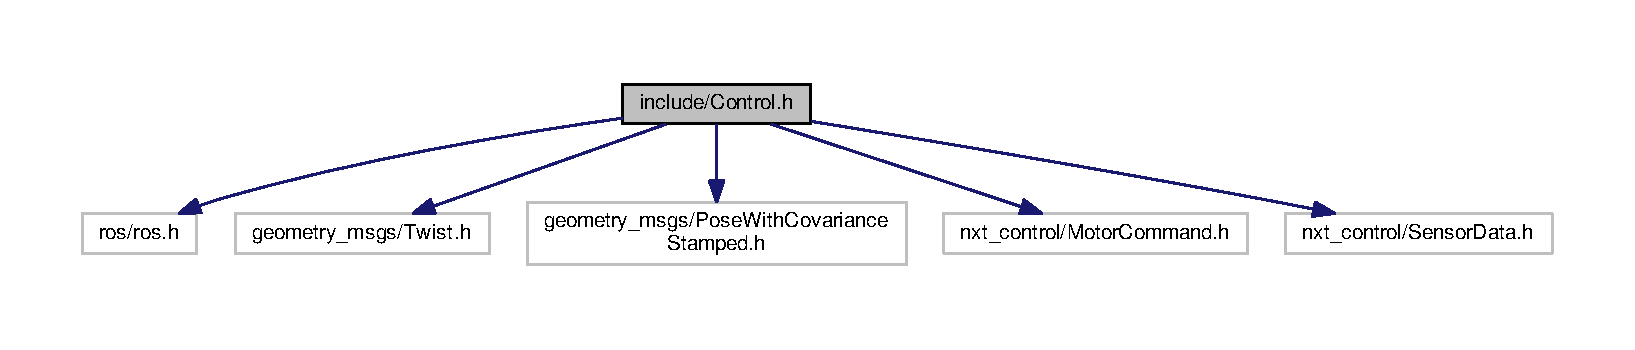
\includegraphics[width=350pt]{Control_8h__incl}
\end{center}
\end{figure}
This graph shows which files directly or indirectly include this file\-:\nopagebreak
\begin{figure}[H]
\begin{center}
\leavevmode
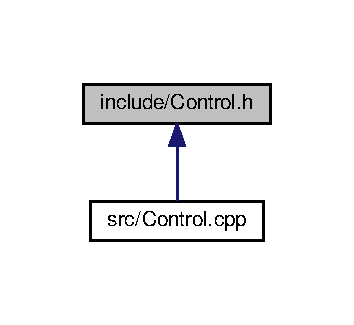
\includegraphics[width=170pt]{Control_8h__dep__incl}
\end{center}
\end{figure}
\subsection*{Classes}
\begin{DoxyCompactItemize}
\item 
class \hyperlink{classControl}{Control}
\item 
struct \hyperlink{structControl_1_1Pose}{Control\-::\-Pose}
\begin{DoxyCompactList}\small\item\em The \hyperlink{structControl_1_1Pose}{Pose} include the 2 d x and x position and the heading th. \end{DoxyCompactList}\end{DoxyCompactItemize}

\hypertarget{cmd__joy_8cpp}{\section{src/cmd\-\_\-joy.cpp File Reference}
\label{cmd__joy_8cpp}\index{src/cmd\-\_\-joy.\-cpp@{src/cmd\-\_\-joy.\-cpp}}
}
{\ttfamily \#include $<$ros/ros.\-h$>$}\\*
{\ttfamily \#include $<$geometry\-\_\-msgs/\-Twist.\-h$>$}\\*
{\ttfamily \#include $<$sensor\-\_\-msgs/\-Joy.\-h$>$}\\*
Include dependency graph for cmd\-\_\-joy.\-cpp\-:\nopagebreak
\begin{figure}[H]
\begin{center}
\leavevmode
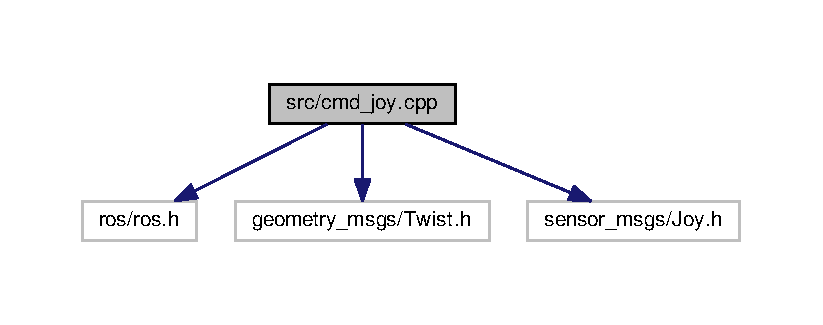
\includegraphics[width=350pt]{cmd__joy_8cpp__incl}
\end{center}
\end{figure}
\subsection*{Classes}
\begin{DoxyCompactItemize}
\item 
class \hyperlink{classcmd__vel__joystick}{cmd\-\_\-vel\-\_\-joystick}
\end{DoxyCompactItemize}
\subsection*{Functions}
\begin{DoxyCompactItemize}
\item 
int \hyperlink{cmd__joy_8cpp_a98135bd506b3ed7bb7fede9ca4af3ed6}{sgn} (double d)
\item 
int \hyperlink{cmd__joy_8cpp_a3c04138a5bfe5d72780bb7e82a18e627}{main} (int argc, char $\ast$$\ast$argv)
\end{DoxyCompactItemize}


\subsection{Function Documentation}
\hypertarget{cmd__joy_8cpp_a3c04138a5bfe5d72780bb7e82a18e627}{\index{cmd\-\_\-joy.\-cpp@{cmd\-\_\-joy.\-cpp}!main@{main}}
\index{main@{main}!cmd_joy.cpp@{cmd\-\_\-joy.\-cpp}}
\subsubsection[{main}]{\setlength{\rightskip}{0pt plus 5cm}int main (
\begin{DoxyParamCaption}
\item[{int}]{argc, }
\item[{char $\ast$$\ast$}]{argv}
\end{DoxyParamCaption}
)}}\label{cmd__joy_8cpp_a3c04138a5bfe5d72780bb7e82a18e627}


Definition at line 91 of file cmd\-\_\-joy.\-cpp.

\hypertarget{cmd__joy_8cpp_a98135bd506b3ed7bb7fede9ca4af3ed6}{\index{cmd\-\_\-joy.\-cpp@{cmd\-\_\-joy.\-cpp}!sgn@{sgn}}
\index{sgn@{sgn}!cmd_joy.cpp@{cmd\-\_\-joy.\-cpp}}
\subsubsection[{sgn}]{\setlength{\rightskip}{0pt plus 5cm}int sgn (
\begin{DoxyParamCaption}
\item[{double}]{d}
\end{DoxyParamCaption}
)}}\label{cmd__joy_8cpp_a98135bd506b3ed7bb7fede9ca4af3ed6}


Definition at line 40 of file cmd\-\_\-joy.\-cpp.


\hypertarget{Control_8cpp}{\section{src/\-Control.cpp File Reference}
\label{Control_8cpp}\index{src/\-Control.\-cpp@{src/\-Control.\-cpp}}
}
{\ttfamily \#include $<$ros/ros.\-h$>$}\\*
{\ttfamily \#include $<$geometry\-\_\-msgs/\-Twist.\-h$>$}\\*
{\ttfamily \#include \char`\"{}geometry\-\_\-msgs/\-Pose\-With\-Covariance\-Stamped.\-h\char`\"{}}\\*
{\ttfamily \#include \char`\"{}sensor\-\_\-msgs/\-Range.\-h\char`\"{}}\\*
{\ttfamily \#include \char`\"{}Control.\-h\char`\"{}}\\*
{\ttfamily \#include $<$tf/transform\-\_\-broadcaster.\-h$>$}\\*
{\ttfamily \#include $<$tf/transform\-\_\-listener.\-h$>$}\\*
{\ttfamily \#include $<$std\-\_\-msgs/\-Bool.\-h$>$}\\*
Include dependency graph for Control.\-cpp\-:\nopagebreak
\begin{figure}[H]
\begin{center}
\leavevmode
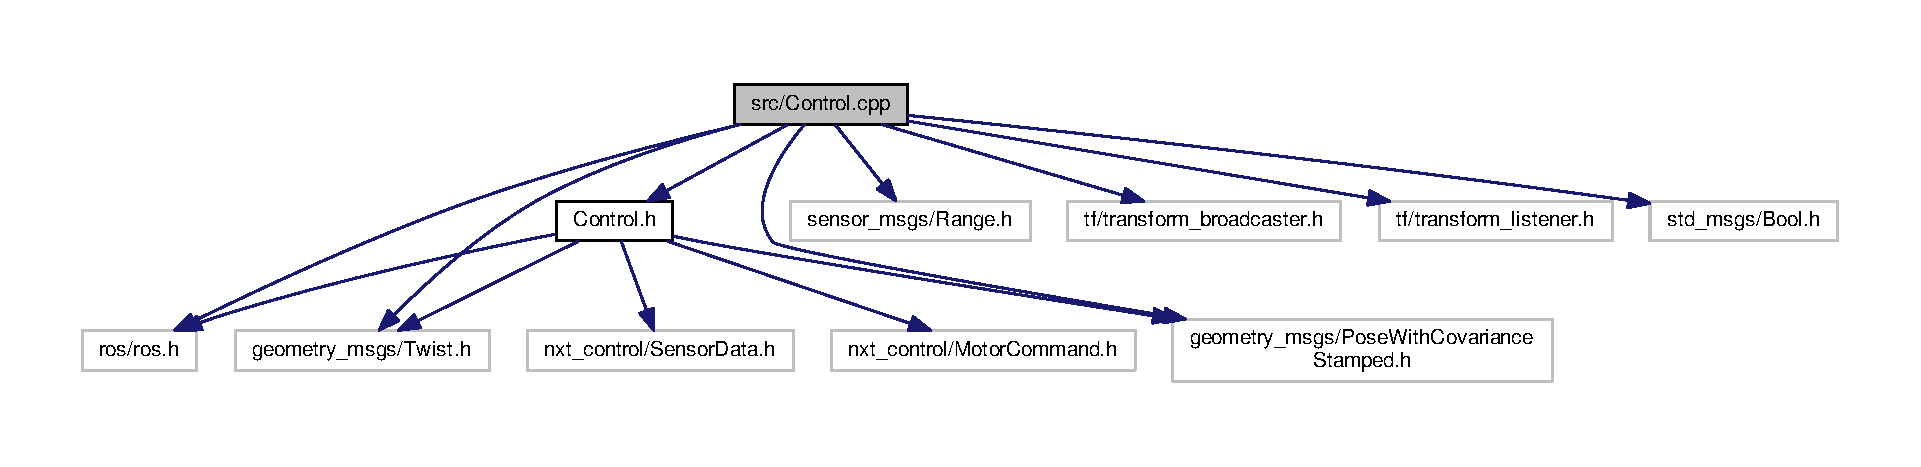
\includegraphics[width=350pt]{Control_8cpp__incl}
\end{center}
\end{figure}
\subsection*{Functions}
\begin{DoxyCompactItemize}
\item 
int \hyperlink{Control_8cpp_a3c04138a5bfe5d72780bb7e82a18e627}{main} (int argc, char $\ast$$\ast$argv)
\end{DoxyCompactItemize}


\subsection{Function Documentation}
\hypertarget{Control_8cpp_a3c04138a5bfe5d72780bb7e82a18e627}{\index{Control.\-cpp@{Control.\-cpp}!main@{main}}
\index{main@{main}!Control.cpp@{Control.\-cpp}}
\subsubsection[{main}]{\setlength{\rightskip}{0pt plus 5cm}int main (
\begin{DoxyParamCaption}
\item[{int}]{argc, }
\item[{char $\ast$$\ast$}]{argv}
\end{DoxyParamCaption}
)}}\label{Control_8cpp_a3c04138a5bfe5d72780bb7e82a18e627}


Definition at line 264 of file Control.\-cpp.


%--- End generated contents ---

% Index
\newpage
\phantomsection
\addcontentsline{toc}{chapter}{Index}
\printindex

\end{document}
